\chapter{Теоретические основы машинного обучения}
\section{Понятие машинного обучения, его типы и задачи}


Машинное обучение само по себе является набором методов для создания моделей, способных решать человеческие задачи. Традиционное программирование предполагает детерминированный выход для каждого набора входных данных. Машинное обучение, напротив, может решать класс задач, для которых соответствие входа и выхода недостаточно хорошо определено \cite{15,22}. 

Обучение под собой подразумевает создание правил, по которым программа будет выдавать ответ. Эти правила можно задавать вручную, рассматривая все возможные варианты. Из-за сложности рассмотрения большого количества вариантов круг задач существенно уменьшается. На выходе получается экспертная система, решающая достаточно точно узкий класс задач. Она получает на вход правила и данные, а на выходе выдает ответы \cite{16,27}.

Благодаря росту объема общедоступных данных в сети Интернет, появился вариант обучить модель не с помощью определения правил, а с помощью метода проб и ошибок. Технически программа получает на вход большое количество данных и ответы для них, а на выходе выдает составленные ею правила, по которым и можно решать необходимые задачи. Такое обучение получило название обучение с учителем. Учителем являетсянабор ответов, сопоставленный с набором входных данных. Такая схема упрощает работу человека в машинном обучении, но взамен требует больших вычислительных ресурсов \cite{13}. 

Также существуют методы обучения без учителя, т.е. без ответов. В таких методах модель обучается только на основе входных данных. Одна из задач машинного обучения это кластеризация данных и ее выполняют с помощью обучения без учителя. Кластеризация подразумевает разделение данных по схожим признакам. Машина должна научится находить общие элементы и сгруппировать по ним набор данных. Также метод понижения размерности без каких-либо ответов на входе \cite{19,26}. Задача этого метода найти такие элементы или характеристики объектов, которые хуже всего описывают их во всем наборе данных и отбросить их. Таким образом вектор признаков станет меньшей размерности. Это помогает модифицировать и упростить другие системы \cite{12,23}. 

Обучение с подкреплением в отличии от предыдущих вариантов обучает на основе информации, собранной при наблюдении за тем, как окружающая среда реагирует на те или иные действия. Этот тип обучения используется в робототехнике. За каждое “действие” программа будет получать “награду”, которая различна для каждых действий. Задачи модели состоит составить такой набор действий, который принесет максимальную награду \cite{8,10}.


\section{Признаки и метрики расстояний}

Для обучения необходимы данные. Но программа не может получить на вход необработанные данные, у нее нет глаз и ушей, она может принимать на вход только определенные математические объекты: числа, векторы, матрицы и графы. 
Главными элементами всех форм представления данных выступают признаки, которые являются наблюдаемыми свойствами объекта \cite{14}. Наборы признаков, которые описывают основные свойства объектов, формируют вектор. 
Вектор признаков описывает упрощенную модель реального объекта, в которой самые незначащие признаки опускаются. Обычно в машинном обучении работает правило: чем больше данных, тем лучше результат,однако, если вектор признаков будет слишком большой размерности, то производительность системы может сильно пострадать \cite{6,24}.

Векторы признаков используются как на этапе обучения, так и на этапе использования программы. Входные данные перед использованием преобразуются в n-мерные векторы признаков, а задача машинного обучения найти наиболее близкие к ним объекты в n-мерном пространстве \cite{11}. Расстояние объектов в пространстве определяется метриками, например Евклидовым расстояние \ref{e:1}:


\begin{equation} \label{e:1}
L_{2} = (\sum (x_{n}-y_{n})^2)^\frac{1}{2},
\end{equation}

где $x_{n}$ координаты одного объекта, а $y_{n}$ второго объекта.
Это $L_{2}$--норма расстояния. Также существуют $L_{0}$,  $L_{1}$, …, $L_{N}$, $L_{\infty}$ нормы расстояний. $L_{0}$--норма смотрит различия в координатах, если многие из координат не совпадают, то объекты считаются достаточно далекими друг от друга. $L_{1}$--норма расстояний является суммой абсолютных разностей координат объекта \ref{e:2}:

\begin{equation}\label{e:2}
L_{1} = \sum |x_{n}-y_{n}|.
\end{equation}

	
Остальные нормы определяются формулой \ref{e:3}: 

\begin{equation}\label{e:3}
L_{N} = (\sum |x_{n}-y_{n}|^N)^\frac{1}{N}.
\end{equation}

	
$L_{\infty}$--норма определяется как наибольшая по модулю величина из всех элементов вектора.
Метрики расстояний помогают также во время обучения, в процессе проверки ответов для дальнейшей корректировки. Выходной вектор на итерации содержит какое-то приближенное значение ответа, это значение необходимо как-то сравнить с готовым, наперед заданным ответом и внести изменение в систему. Неплохим способом их сравнить — найти расстояние между ними. Сравнивая это расстояние для различных параметров внутри модели, можно получить функцию расстояния(функцию ошибки) — $E(w_{n})$, где $w_{n}$ — набор изменяемых параметров внутри модели. Теперь становится возможным минимизировать ошибку. Для этого необходимо найти минимум этой функции, например алгоритмом градиентного спуска \cite{5, 7}.


\section{Перцептрон, простая модель обучения}


Перцептрон — кибернетическая модель человеческого мозга, которая теоретически описывает достаточно упрощенный процесс мышления. В основе этой модели лежат узлы связей — нейроны, которые являются простым подобием нейронов головного мозга (органических клеток). Также как и органические нейроны, искусственные имеют различные связи между собой (рисунок \ref{fig:1}) \cite{3,9}. 

\begin{figure}[ht] 
  \center
  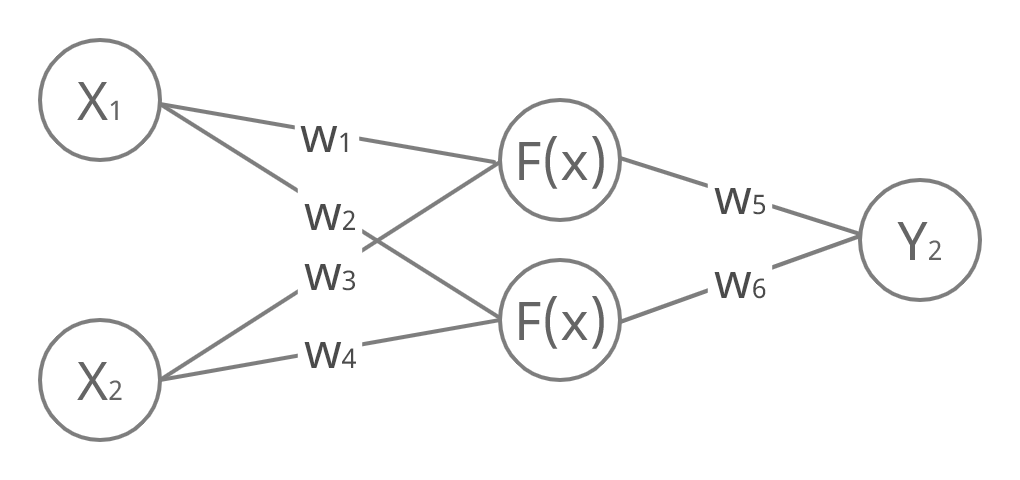
\includegraphics [scale=0.4] {img/Perceptron.png}
  \caption{Пример простой модели перцептрона из трех слоев} 
  \label{fig:1}  
\end{figure}

В данном примере $X_{1}$ и $X_{2}$ являются элементами вектора признаков $(X_{1},  X_{2})$. 
$w_{1}$, $w_{2}$, $w_{3}$, $w_{4}$, $w_{5}$, $w_{6}$ — изменяемые параметры модели (веса), они описывают степень связи между нейронами, нахождение значений весов, при которых программа будет исправно работать — одна из задач машинного обучения. $F(x)$ — функция активации нейронного слоя.  Она позволяет преобразовывать данные с предыдущих слоев в сигнал для последующих. $Y_{1}$ — является одномерным вектором ответов \cite{4}. Сравнивая его с готовыми ответами можно вычислить ошибку $E$. Значение входных сигналов считается путем простого перемножения вектора выходных сигналов предыдущего слоя на матрицу весов между слоями. Теперь можно вычислить локальный градиент нейрона $\delta = E \cdot F'(x)$ и скорректировать веса, например для $w_{5}$ \ref{e:4}:

\begin{equation} \label{e:4}
w_{5} = w_{5} - \lambda \delta F(w_{1}X_{1} + w_{3}X_{2}),
\end{equation}


где $\lambda$ — шаг сходимости алгоритма обучения, это некоторый коэффициент который подбирается вручную.

Такой подход к корректировке весов и уменьшению ошибки называется методом обратного распространения ошибки, который основан на методе градиентного спуска \cite{1}. И все проблемы градиентного спуска ложатся и на алгоритм обратного распространения ошибки. Например попадание в локальный минимум. Общего решения для такой проблемы нет, поэтому на практике следует запускать алгоритмы обучения с разными значениями начальных коэффициентов $w_{n}$. Также возможна проблема низкой скорости сходимости градиентного спуска на пологих участках функции. Для этого используют алгоритмы оптимизации, такие как ускоренные градиенты Нестерова или метод Adam \cite{2}.